%!TEX root = ../thesis.tex
%*******************************************************************************
%****************************** Third Chapter **********************************
%*******************************************************************************
\chapter{The dynamic sRNA profile and inheritance of paternal epigenetic modifications post-fertilisation in the embryo of \textit{Marchantia polymorpha}}

% **************************** Define Graphics Path **************************
\ifpdf
    \graphicspath{{Chapter3/Figs/Raster/}{Chapter3/Figs/PDF/}{Chapter3/Figs/}}
\else
    \graphicspath{{Chapter3/Figs/Vector/}{Chapter3/Figs/}}
\fi


\section{Abstract}

\section{Introduction}

Recently, our group has shown that during spermatogenesis, there extensive DNA methylation reprogramming in Marchantia. As well as the deposition of 5-methylcytosine (5mC), there is an additional wave of DNA methylation reprogramming whereby N4-methylcytosine (4mC) - an epigenetic modification previously only found in prokaryotes – is deposited at the majority of CG cites across the genome \citep{RN189}. 

Data from mature embryo reveals that this 4mC methylation is not present. Several hypotheses could explain why this happens. The most likely is that following fertilisation, paternal epigenetic marks are lost passively through cell division. Alternatively, the marks could be maintained through the first few cell divisions and then are actively or passively lost. We also know that the pronuclei take 3 days to fuse \citep{RN139}, so it is also possible that removing paternal epigenetic marks is required for zygote formation. 

Therefore, my project here will help complement the work that has already been done on 4mC methylation in Marchantia; please see our lab’s preprint for other details of this project \citep{RN189}. Namely, I have already managed to isolate and image embryos 12 days after fertilisation (DAF), and I plan to isolate and stage embryos that are as young as possible to make sure that we can detect 4mC signals if paternal epigenetic marks are maintained through zygote formation but are passively lost during cell division.

\subsection{Overview of DNA methylation in the germline of Marchantia polymorpha}

Recently, our group has shown that during Marchantia spermiogenesis extensive DNA methylation reprogramming occurs. As well as the deposition of 5-methylcytosine (5mC), there is an additional wave of DNA methylation reprogramming whereby N4-methylcytosine (4mC) – an epigenetic modification previously only found in prokaryotes – is deposited at the majority of CG cites across the genome \citep{RN189}.

However, this methylation is absent in the mature embryo (containing over 1000 cells). The exact point in time when 4mC methylation disappears post-fertilisation remains unknown, as does whether the paternal genome retains any 4mC marks during the early stages of zygotic development. The first division of the zygote in Marchantia takes place around 4 days post-fertilisation1 which suggests that 4mC may be required to be actively removed for pronuclear fusion to occur. This aligns with the observed phenotype where embryos fertilised by Mpdn4mt1 sperm develop more rapidly, though this phenotype needs to be confirmed during early embryonic development. Alternatively, 4mC methylation could be lost passively following fertilisation through dilution by cell division, or actively removed post-fertilisation for DNA replication or cell division to function normally. 4mC may also be crucial in the correct genome dosage/transcriptional activity during early embryonic development. 

In Arabidopsis, 5mC methylation is lost actively to maintain homeostasis of DNA methylation levels through several DNA glycosylases, including ROS1 \citep{RN168}. Therefore, the orthologs of ROS1 in Marchantia, MpROS1a and MpROS1x (located on the female sex chromosome) offer possible candidates for erasing paternal 4mC methylation as they are expressed in the sperm \citep{RN212} and mature eggs/embryos \citep{RN257} respectively.

It has also recently been shown that other epigenetic marks, namely the heterochromatic histone modification H3K27me3 is deposited at the pronuclear stage exclusively on the paternal genome and causes the repression of the paternal genome persisting until the conclusion of embryogenesis \citep{RN160}. In contrast, in mammalian germlines, H3K27me3¬ mediated imprinting is limited to a few loci within the female gamete \citep{RN172}.

Hence, investigating the methylation profiles of early Marchantia embryos during the first zygotic divisions and examining the early developmental phenotype of Mpdn4mt1 mutants will complement our previous work, expanding our understanding of how paternal DNA methylation affects early embryonic development.

\section{Developmental phenotype of Mpdn4mt1 mutant embryos}

\begin{figure}[htbp!] 
\centering    
    \includegraphics[width=1\textwidth]{Chapter3/Figs/Figure1_eggs_and_embryos.pdf}
\caption{\textbf{Live cell imaging of the developmental stages of \textit{M. polymorpha} embryos}}
\label{fig:egg_embryo}
\captionsetup{font=small}
    \caption*{Unstained egg cell (first row), DAPI stained egg cell (second row), and embryos 8 days (third row), and 10 days (fourth row) after fertilisation. Scale bar 10$\mu$m}
\end{figure}

\begin{figure}[htbp!] 
\centering    
    \includegraphics[width=1\textwidth]{Chapter3/Figs/Figure2_Reporter_line_gemmae_screening.pdf}
\caption{\textbf{Gemmae screening of constitutively expressed nuclear reporter lines}}
\label{fig:gemma:screen}
\captionsetup{font=small}
    \caption*{Nuclear signal of tdTomato or citrine (second column, red or yellow respectively, white arrows) in gemmae, driven by either 35S constitutive promoter (first row) native constitutive promoter EF$\alpha$ (second and third rows). Scale bar 10$\mu$m.}
\end{figure}

\begin{figure}[htbp!] 
\centering    
    \includegraphics[width=1\textwidth]{Chapter3/Figs/Figure3_Reporter_line_antheridia.pdf}
\caption{\textbf{The tdTomato based nuclear reporter lines are expressed in the antheridia}}
\label{fig:antheridia_screen}
\captionsetup{font=small}
    \caption*{Nuclear signal of tdTomato or citrine (second column, red or green respectively) in the antheridiophore, driven by either 35S constitutive promoter (first row) native constitutive promoter EF$\alpha$ (second and third rows). Scale bar 10$\mu$m.}
\end{figure}

\begin{figure}[htbp!] 
\centering    
    \includegraphics[width=1\textwidth]{Chapter3/Figs/Figure4_reporter_line_malevsfemale.pdf}
\caption{\textbf{Tak1 male nuclear reporter lines crossed to Tak2 females have no nuclear expression in the embryo}}
\label{fig:malevsfemale}
\captionsetup{font=small}
    \caption*{Nuclear signal of tdTomato (second column, red, white arrows) in embryos crossing EF$\alpha$::tdTomato-NLS Tak1 male to WT Tak2 female, 3 days (first row) and 16 days (second row) after fertilisation. Expression of EF$\alpha$::tdTomato-NLS (third row) and  35S::tdTomato-NLS (fourth row) in WT female thallus. Scale bar 10$\mu$m.}
\end{figure}

\begin{figure}[htbp!] 
\centering    
    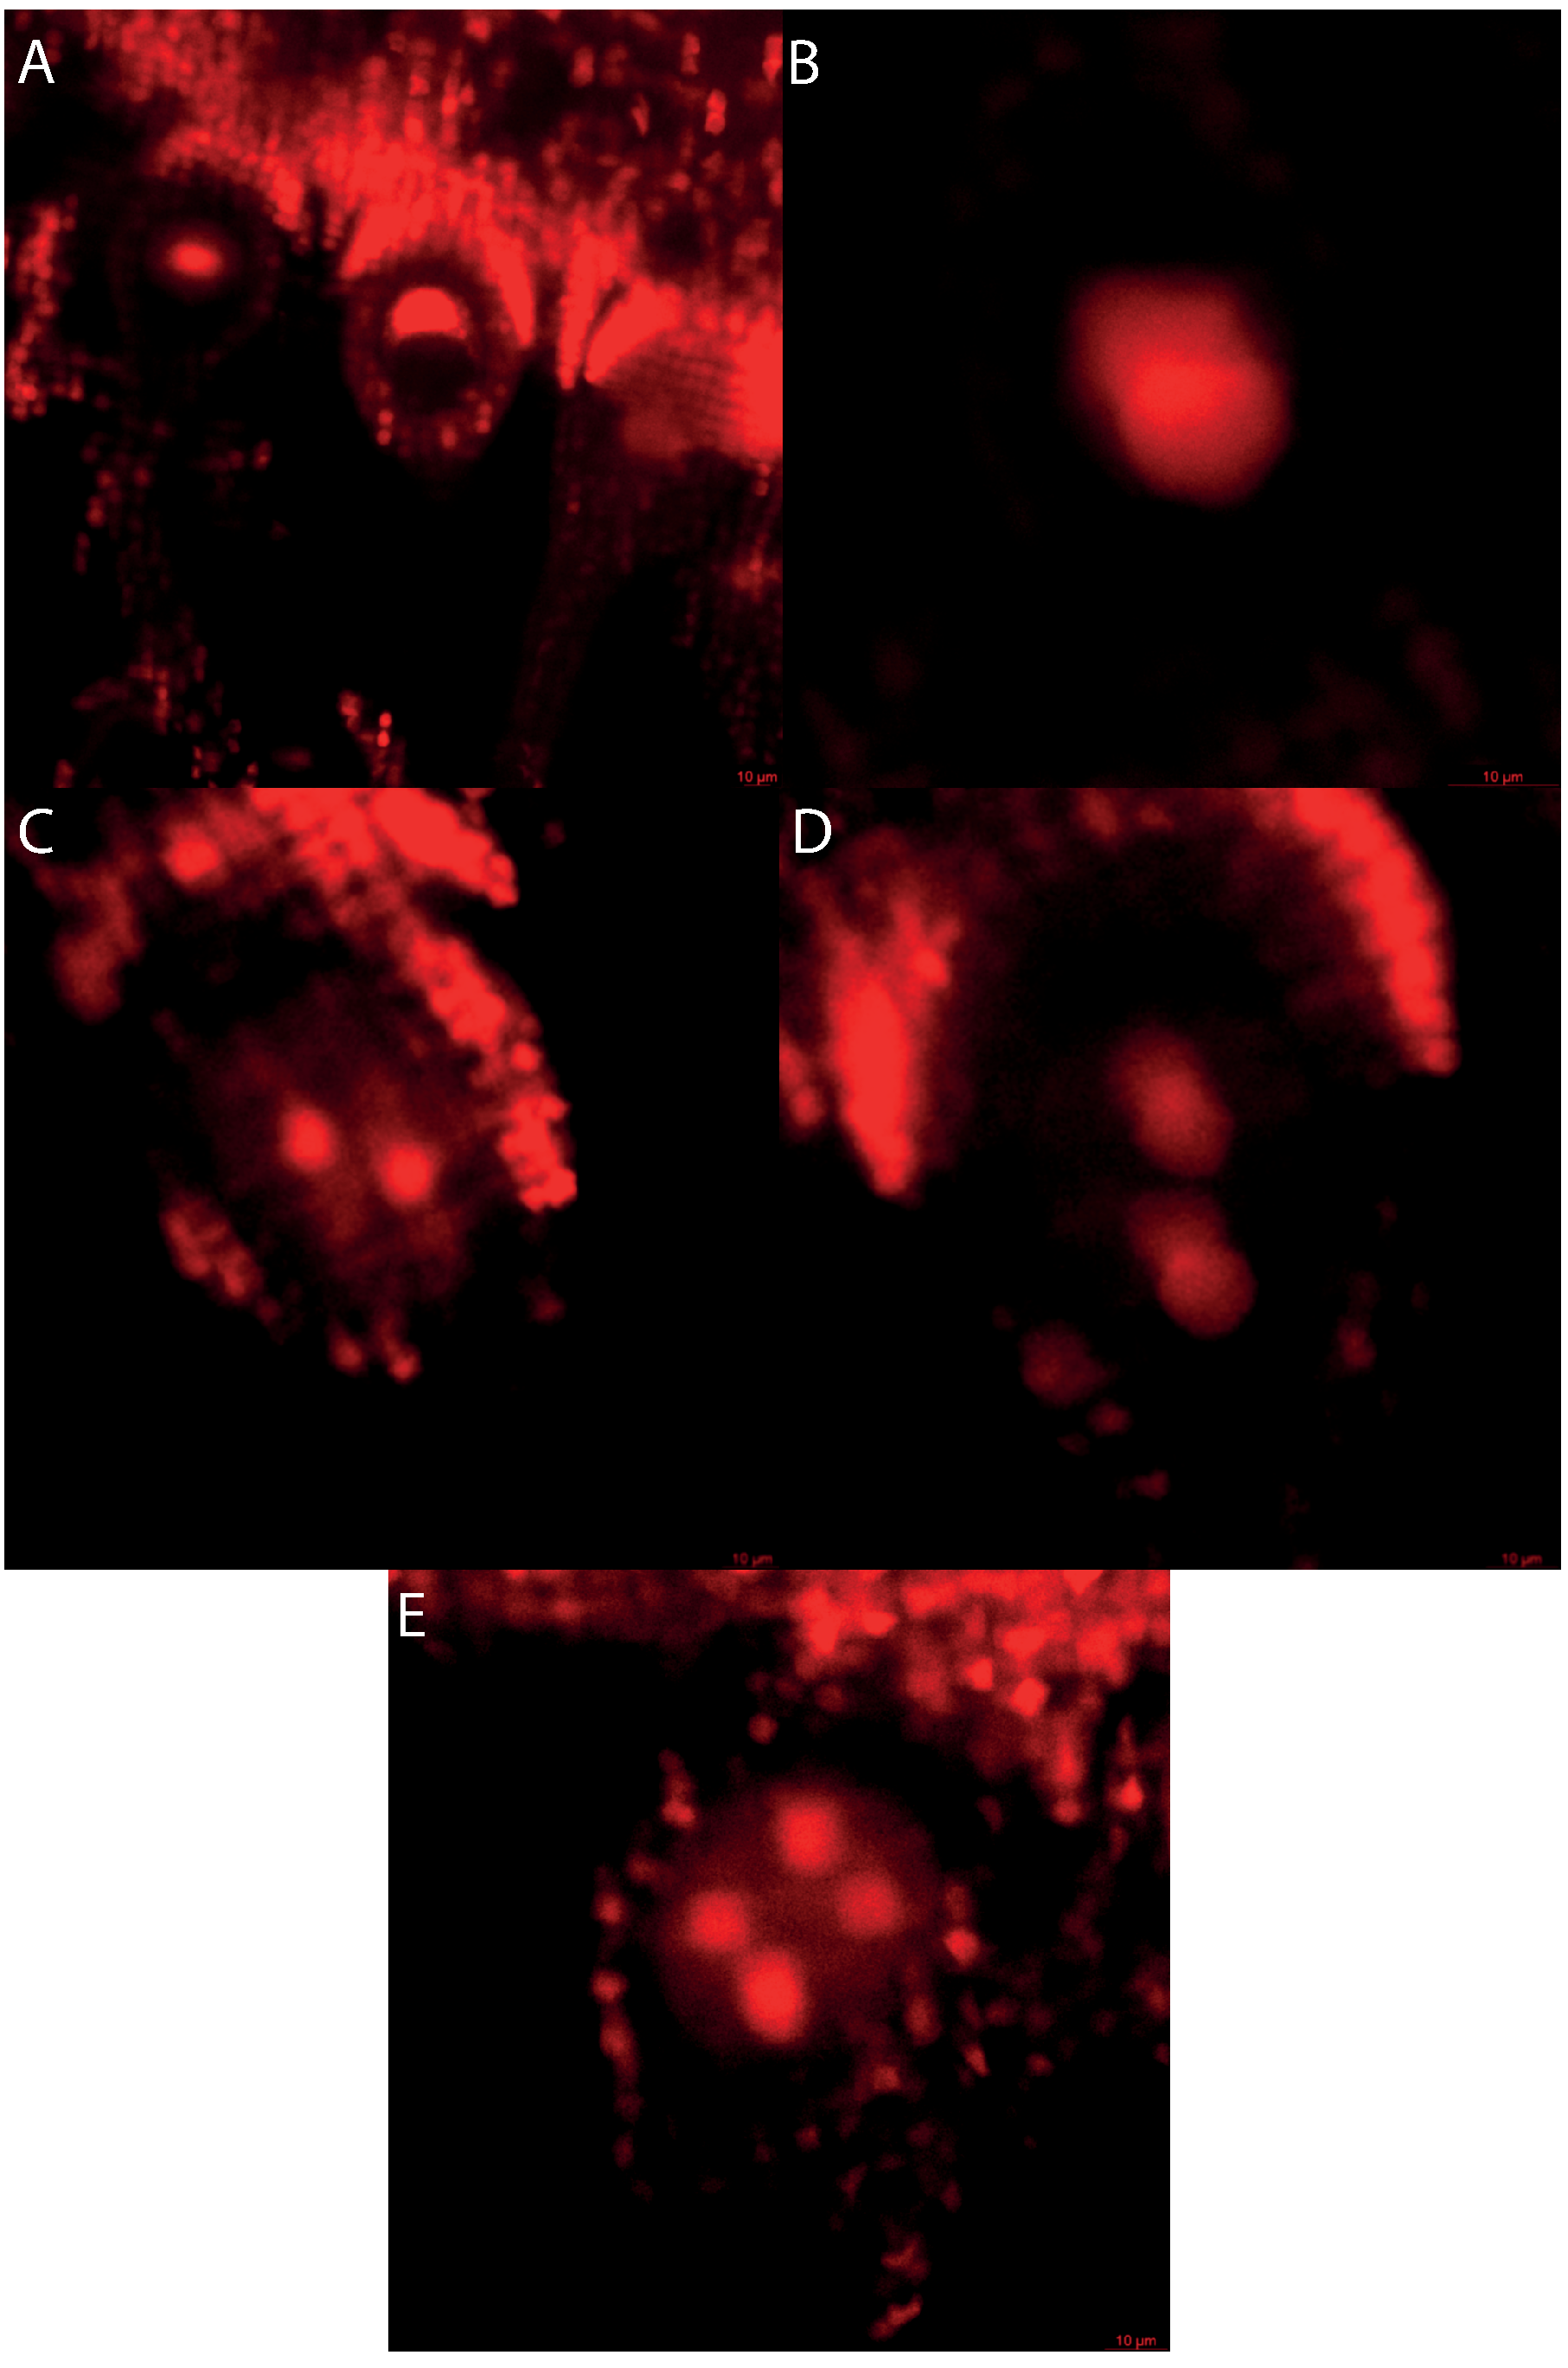
\includegraphics[width=1\textwidth]{Chapter3/Figs/Figure5_Developmental_stages.pdf}
\caption{\textbf{Developmental stages of the early embryo (Tak1 male x EF$\alpha$::tdTomato-NLS WT female)}}
\label{fig:dev_stages}
\captionsetup{font=small}
    \caption*{(A) Zygote (B) Zygote dividing (C) Two-cell stage (D) Two-cell embryo dividing (E) Four-cell stage. Scale bar 10$\mu$m.}
\end{figure}

\begin{figure}[htbp!] 
\centering    
    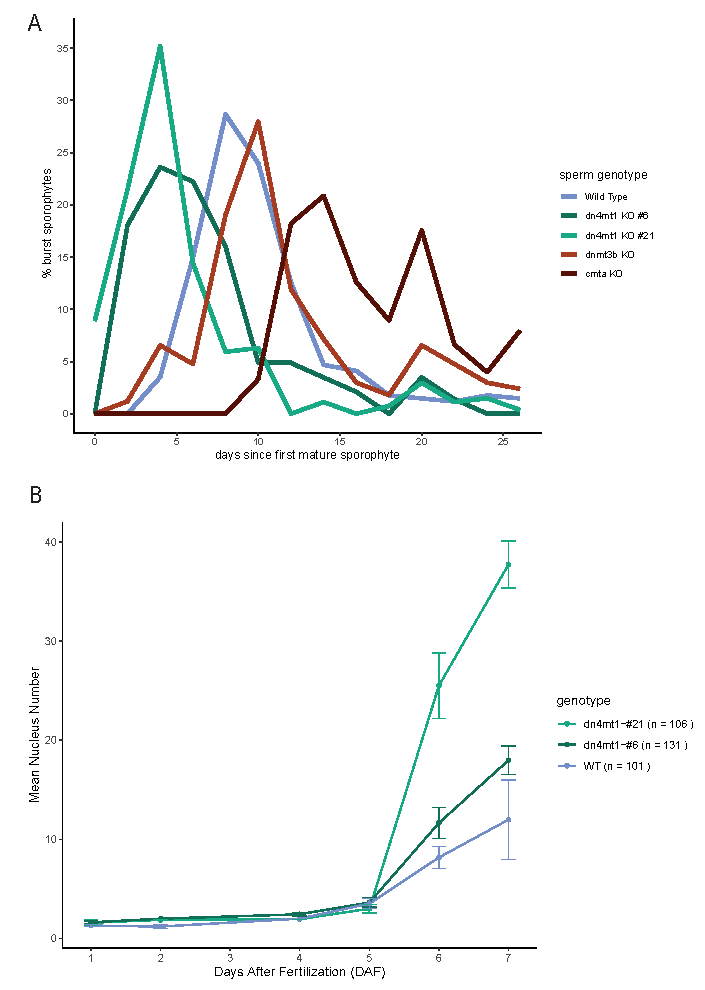
\includegraphics[width=1\textwidth]{Chapter3/Figs/Figure6_burstpeak_nuclei_number.pdf}
\caption{\textbf{Embryos fertilised by \textit{dn4mt1} knockout sperm develop more rapidly than WT}}
\label{fig:burstpeak}
\captionsetup{font=small}
    \caption*{(A) Total percentage of burst sporophytes every day since first mature sporophyte, fertilised with wild type sperm (blue), two independent lines of \textit{dn4mt1} knockout sperm (\#6 dark green, \#21 light green) or 5mC (\textit{cmta} (dark brown) or \textit{dnmt3B}) knockout sperm (light brown). (B) Mean nucleus number of embryos from 1-7 days after fertilisation, fertilised by wild type (blue), \textit{dn4mt1} knockout \#6 (dark green), or \textit{dn4mt1} knockout \#21 (light green) sperm. }
\end{figure}

\begin{figure}[htbp!] 
\centering    
    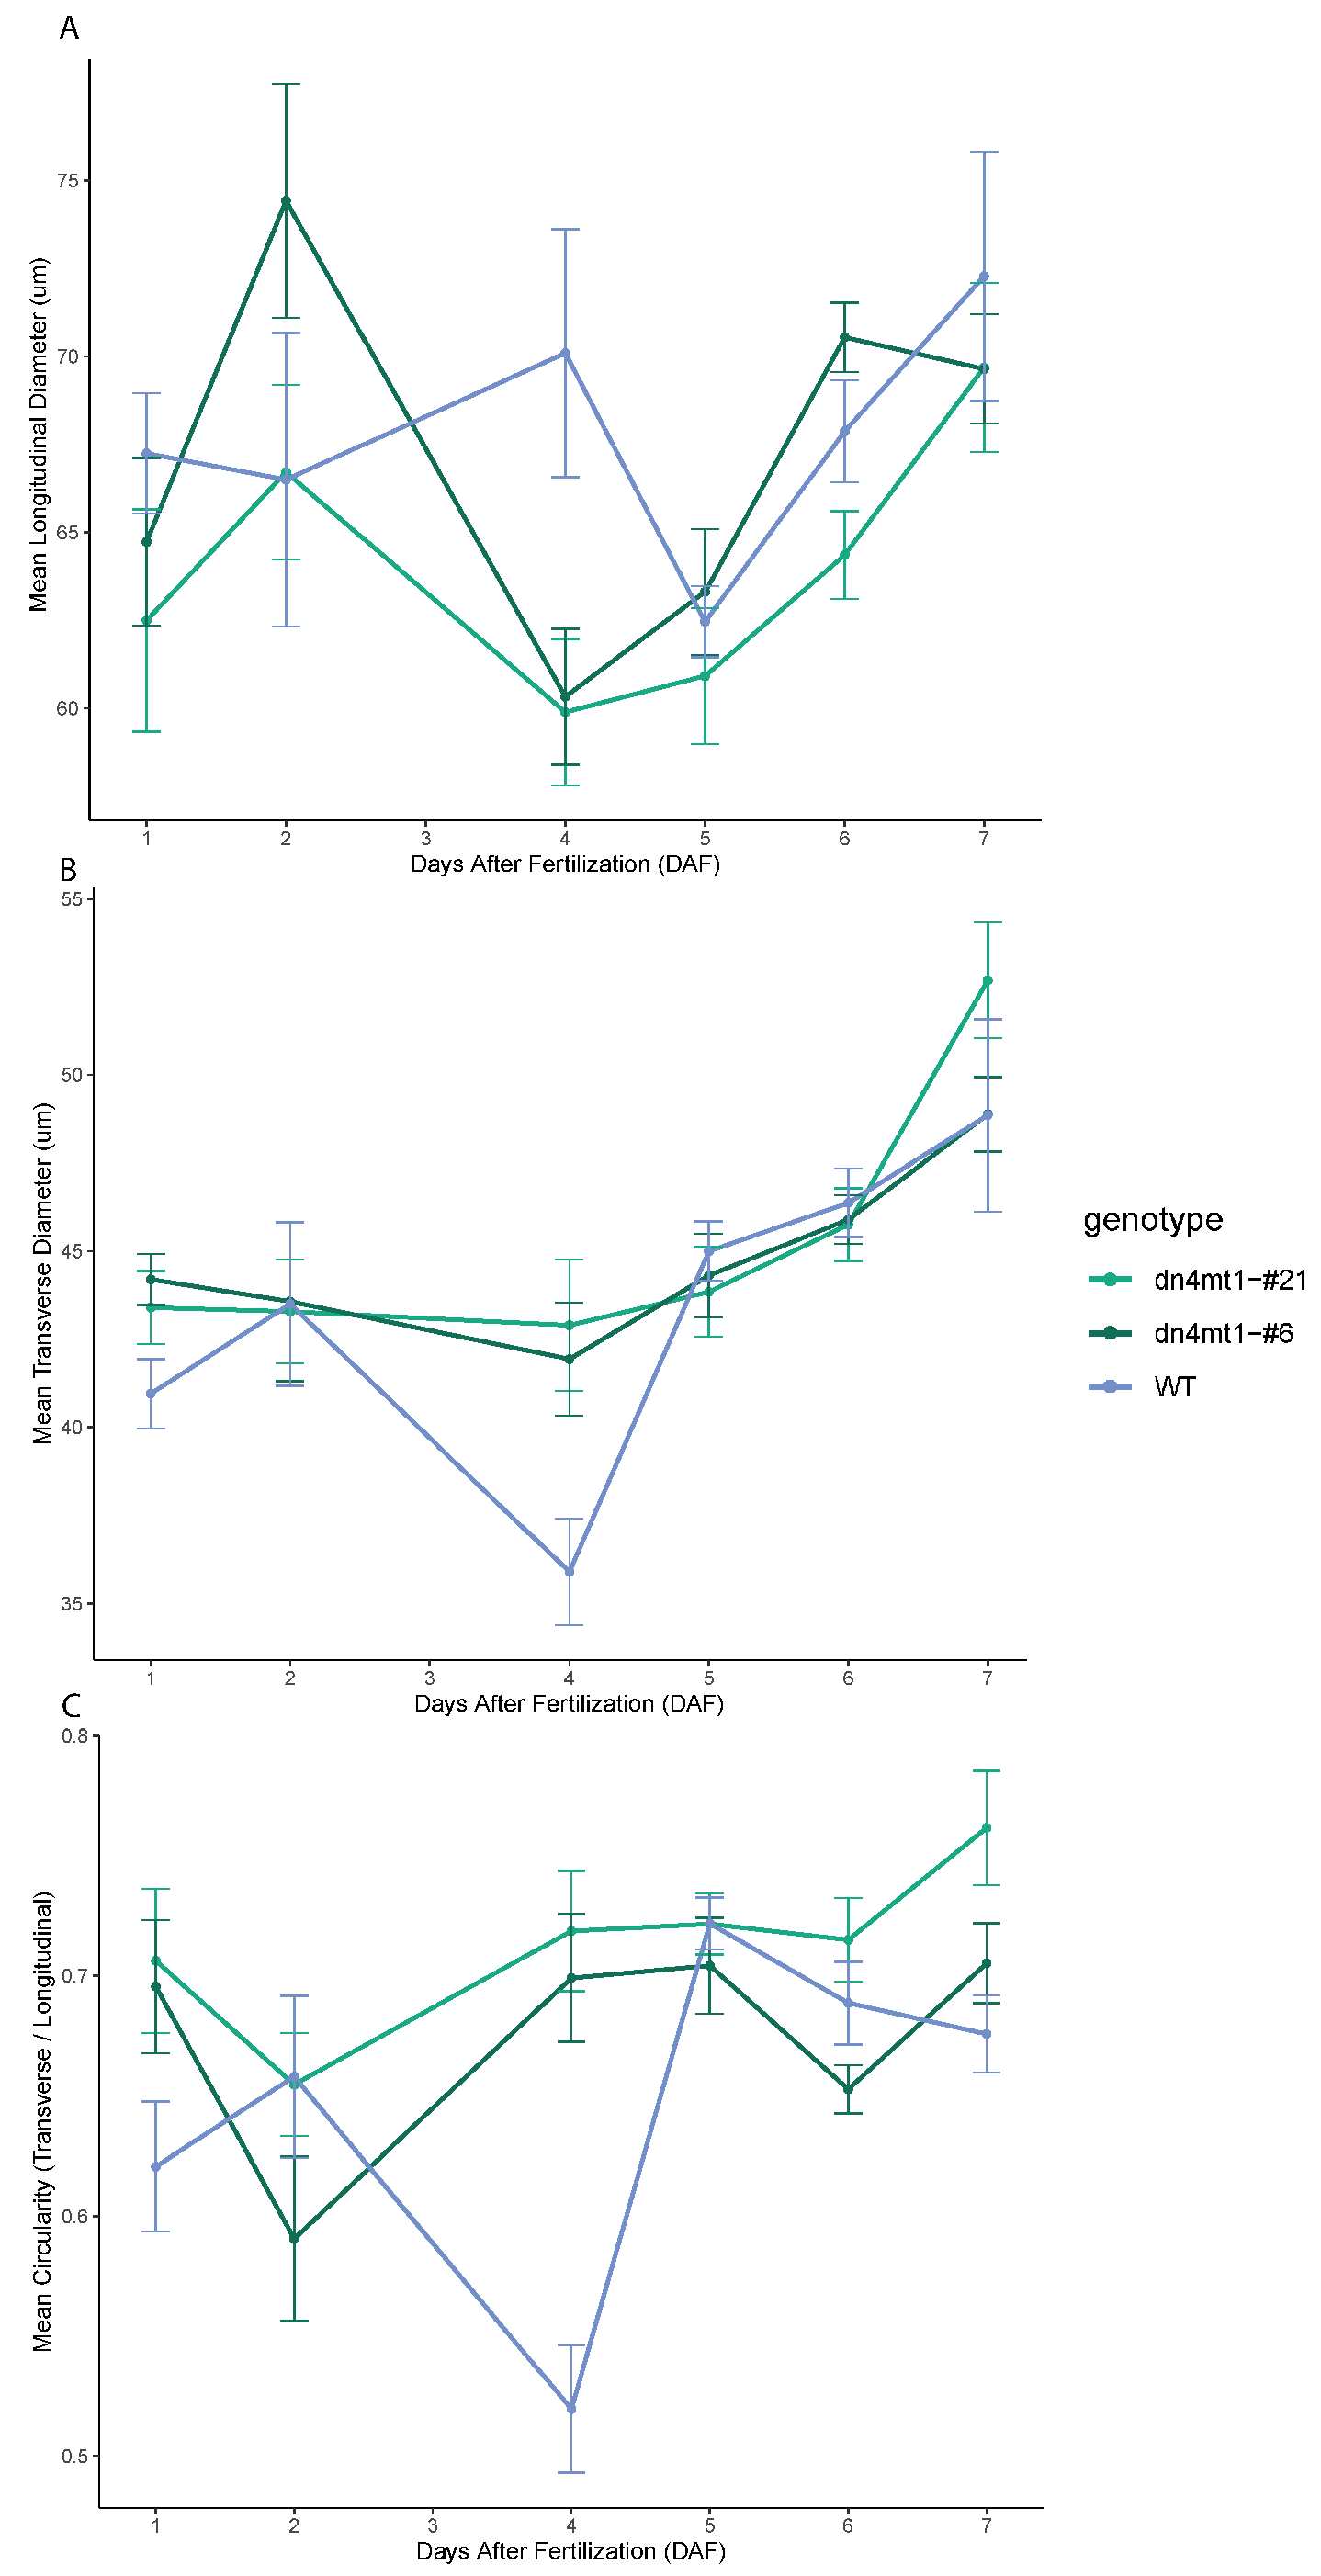
\includegraphics[width=0.75\textwidth]{Chapter3/Figs/Figure7_circularity.pdf}
\caption{\textbf{Embryos fertilised by \textit{dn4mt1} knockout sperm elongate earlier and tend mroe circular earlier than those fertilised by wild type sperm}}
\label{fig:circularity}
\captionsetup{font=small}
    \caption*{(A) Mean longitudinal diameter, (B) Mean transverse diameter, (C) Mean circularity of embryos 1-7 days after fertilisation, fertilised by wild type (blue), \textit{dn4mt1} knockout \#6 (dark green), or \textit{dn4mt1} knockout \#21 (light green) sperm.}
\end{figure}


\section{AMD-seq of early Marchantia embryos}

\begin{figure}[htbp!] 
\centering    
    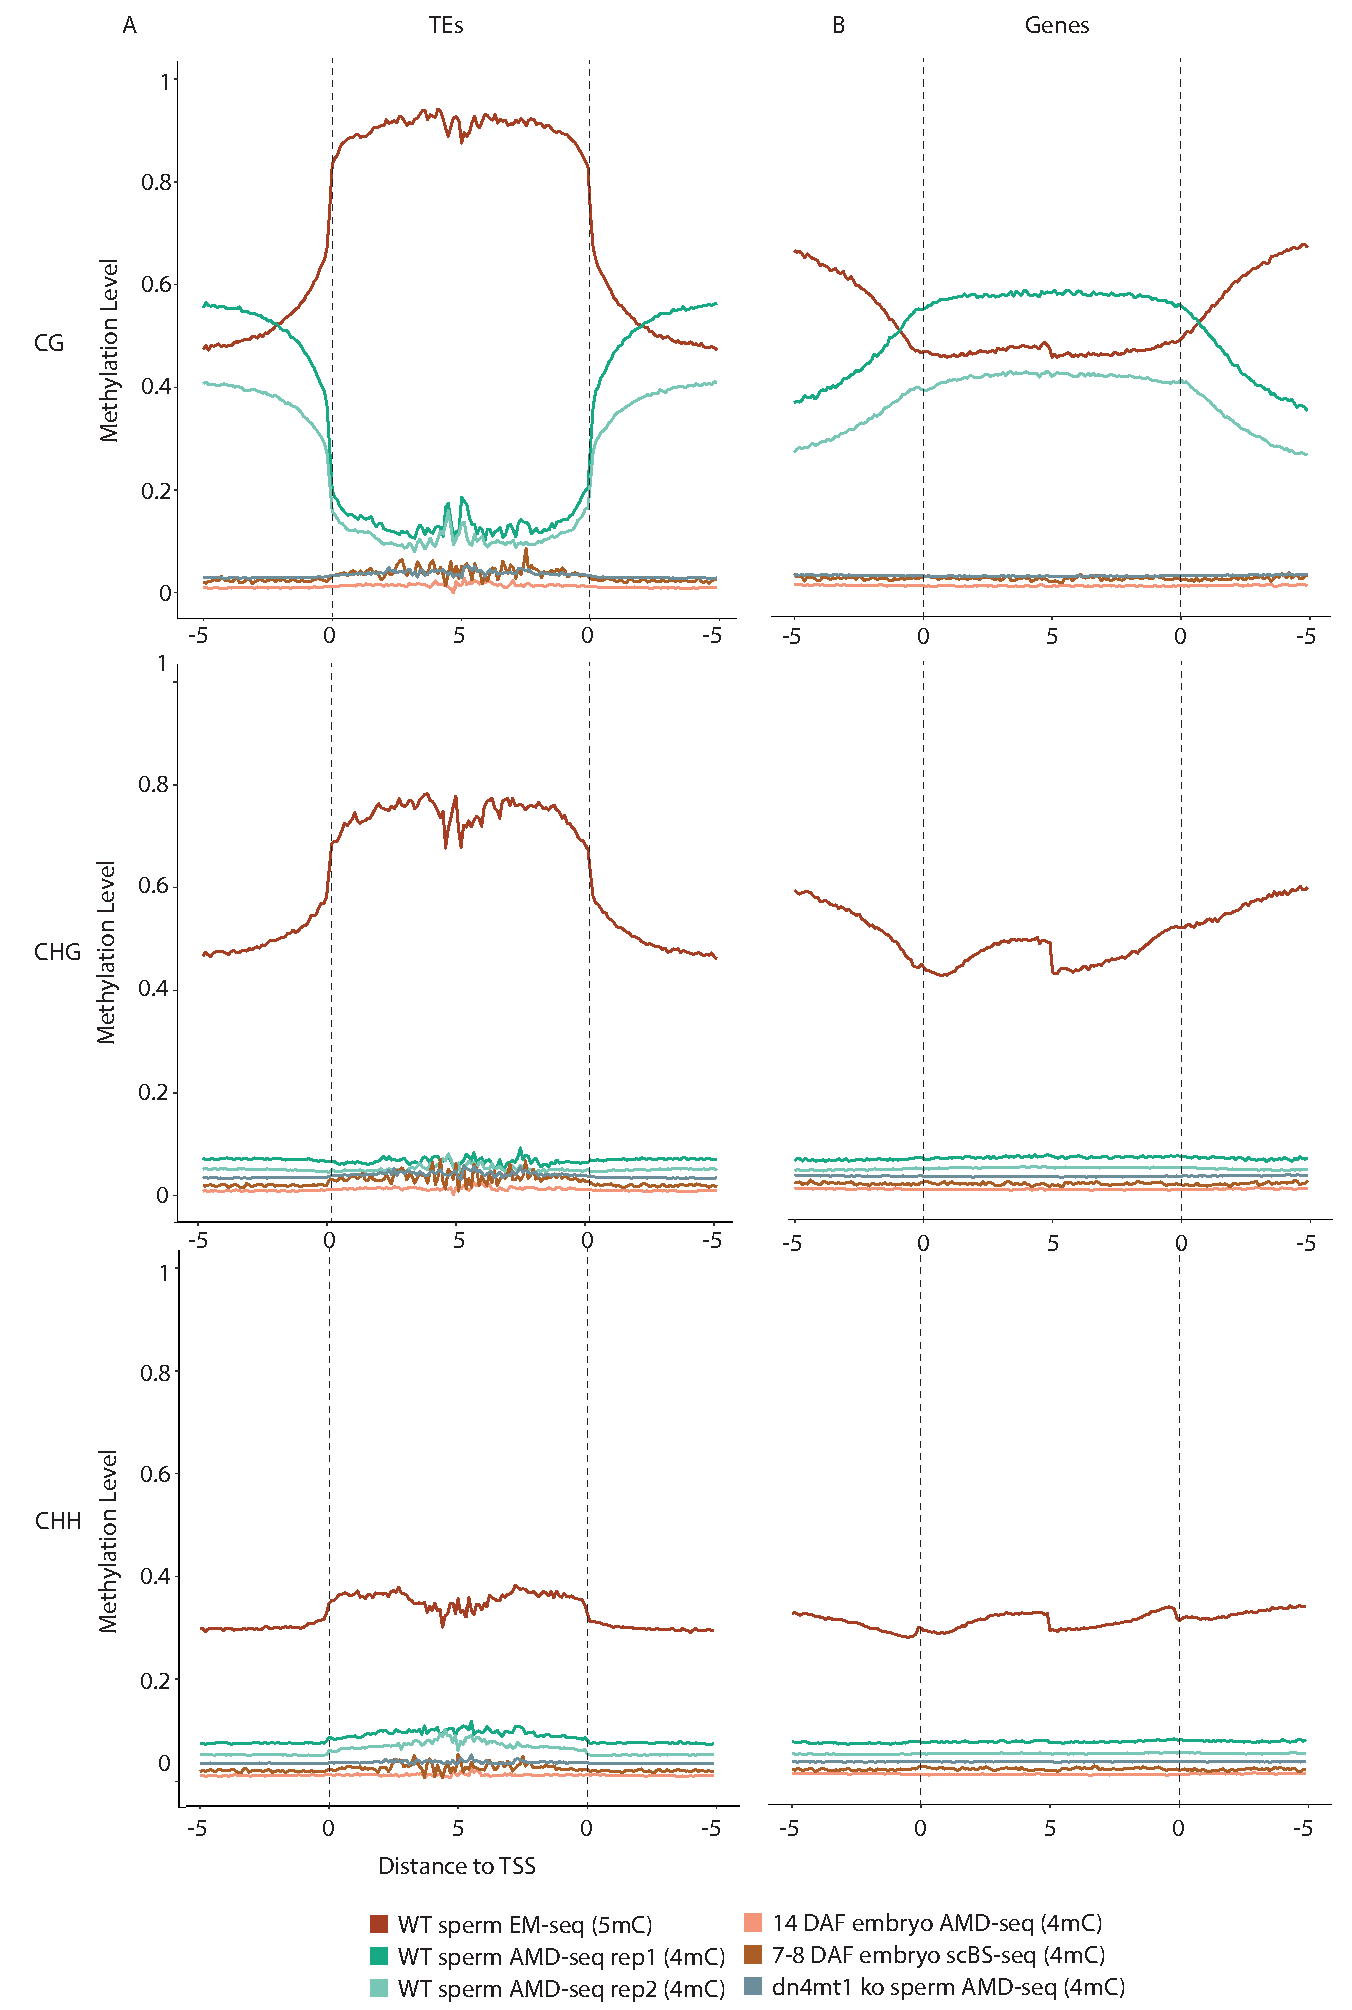
\includegraphics[width=1\textwidth]{Chapter3/Figs/Figure8_ends_analysis.pdf}
\caption{\textbf{4mC methylation occurs in the CG context and is enriched in genic regions and outside of TEs, while 5mC methylation is largerly confined to TEs}}
\label{fig:ends_analysis}
\captionsetup{font=small}
    \caption*{Panel showing 4mC and 5mC methylation across TEs (A) and Genes (B) in CG (first row), CHG (second row) and CHH (third row) sequence contexts in wild type sperm \textit{dn4mt1 sperm}, the embryo 7-8 and 14 days after fertilisation.}
\end{figure}

\begin{table}[htbp!]
\centering
\label{tab:methylation_levels}
\captionsetup{font=small}
\begin{tabular}{|p{5cm}|c|c|c||c|c|c|}
\hline
\multirow{2}{*}{\makecell{Methylation context}} & \multicolumn{3}{c||}{Overall} & \multicolumn{3}{c|}{Genes} \\
\cline{2-7}
 & CG & CHG & CHH & CG & CHG & CHH \\
\hline
WT sperm AMD seq rep1 & 0.467 & 0.071 & 0.075 & 0.559 & 0.071 & 0.072 \\
WT sperm AMD seq rep2 & 0.341 & 0.050 & 0.051 & 0.404 & 0.051 & 0.049 \\
dn4mt1 ko sperm & 0.031 & 0.035 & 0.033 & 0.029 & 0.034 & 0.033 \\
14 DAF embryo & 0.011 & 0.009 & 0.009 & 0.009 & 0.008 & 0.008 \\
7-8 DAF embryo & 0.027 & 0.021 & 0.019 & 0.024 & 0.020 & 0.020 \\
\hline
\multicolumn{7}{|l|}{Theoretical methylation levels} \\
\hline
Zygote & 0.202 & 0.030 & 0.031 & 0.241 & 0.030 & 0.030 \\
16 cell embryo  & 0.013 & 0.016 & 0.015 & 0.015 & 0.015 & 0.015 \\
32 cell embryo & 0.006 & 0.007 & 0.007 & 0.008 & 0.007 & 0.007 \\
\hline
\end{tabular}
\caption{\textbf{Methylation levels across WT sperm, \textit{dn4mt1} sperm and the early embryo}}
\end{table}

\begin{figure}[htbp!] 
\centering    
    \includegraphics[width=1\textwidth]{Chapter3/Figs/Figure9_H3K27me3.pdf}
\caption{\textbf{H3K27me3 levels are elevated in the paternal genome and correlate with the presence of 5mC over genes}}
\label{fig:h3k27me3}
\captionsetup{font=small}
    \caption*{Heatmaps showing the relative H3K27me3 levels in Marchantia embryos over the genes and TEs in the paternal and maternal genomes.}
\end{figure}


\section{sRNA analysis}
\section{Source of sRNAs in the sporophyte (paternal sRNAs with genome shut down?}
\subsection{Mismatch tageting \textit{de novo} methylation (SLMs)}

\begin{figure}[htbp!] 
\centering    
    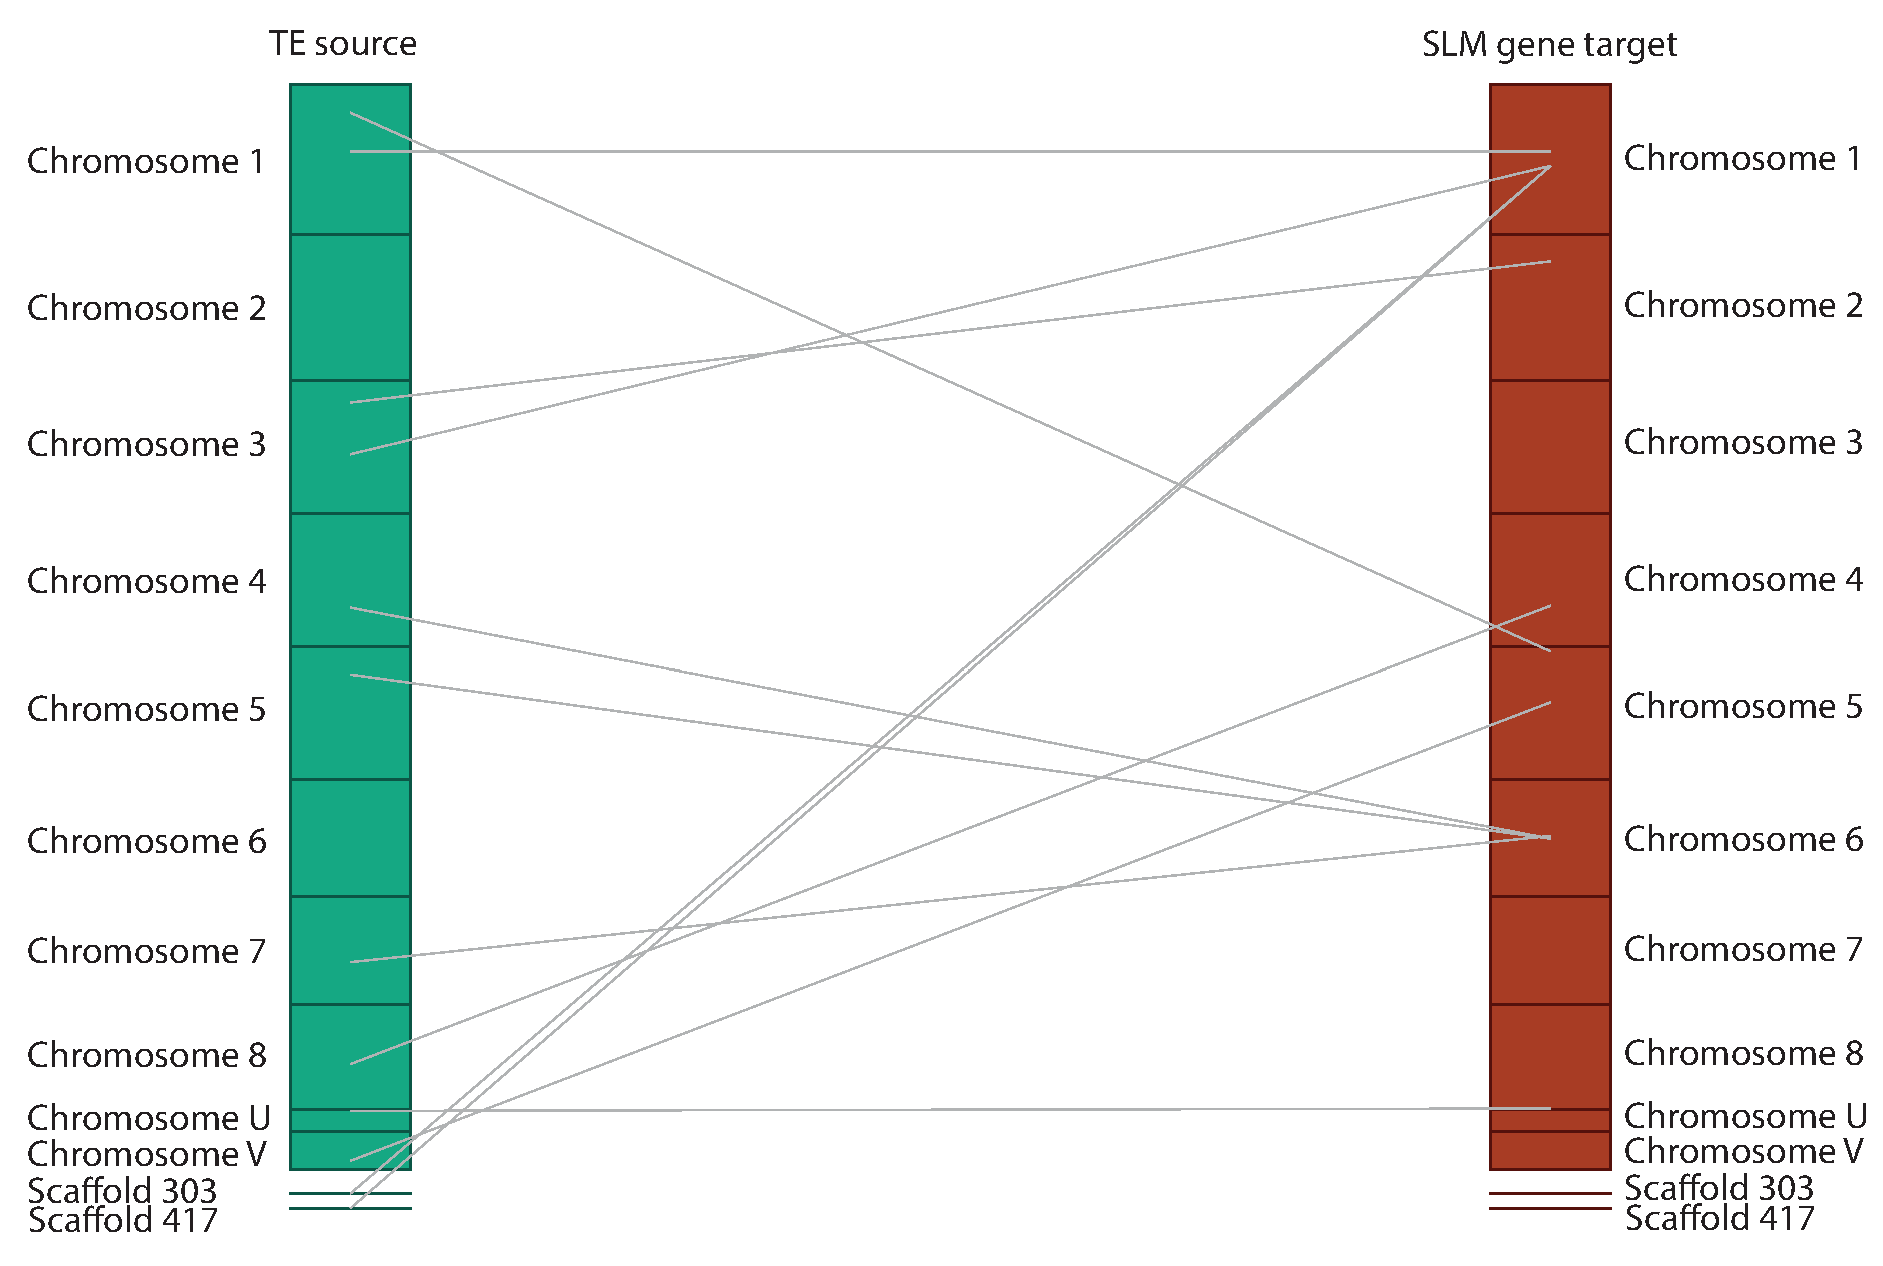
\includegraphics[width=1\textwidth]{Chapter3/Figs/Figure10_SLM_source_target.pdf}
\caption{\textbf{TE loci produce 24nt sRNA that target genic loci for methylation with mismatch targeting}}
\label{fig:SLM_targeting}
\captionsetup{font=small}
    \caption*{Locations of TE source loci (left, green) connected to genic target loci (right, brown)}
\end{figure}

\begin{figure}[htbp!] 
\centering    
    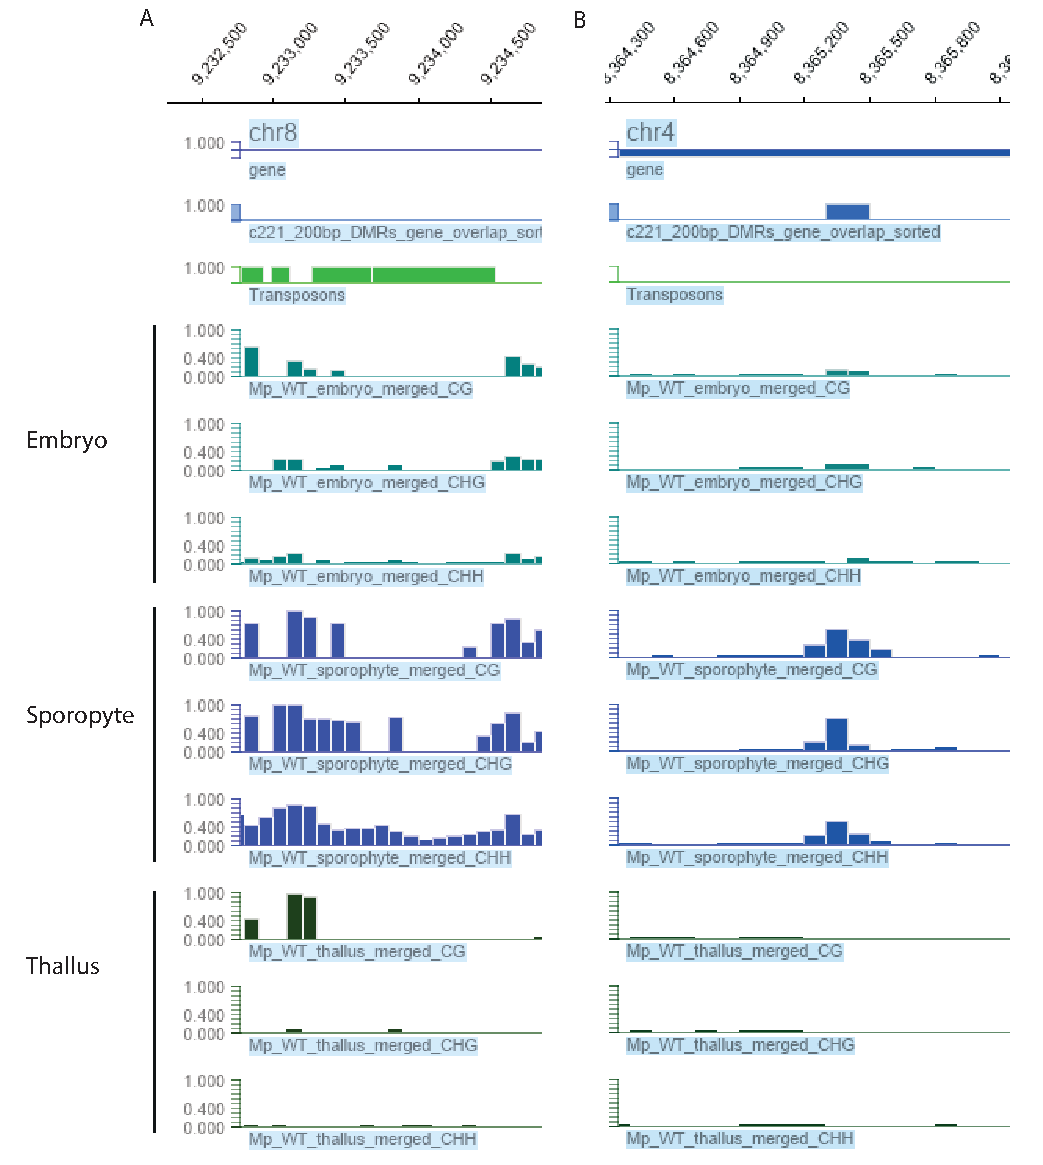
\includegraphics[width=1\textwidth]{Chapter3/Figs/Figure11_pairs_examples.pdf}
\caption{\textbf{Example of a TE  source and SLM target that gain methylation in the sporophyte}}
\label{fig:TE_SLM_pairs}
\captionsetup{font=small}
    \caption*{MMethylaiton levels in (A) TE source and (B) SLM target pair in CG, CHG and CHH sequence contexts in embryo, sporophyte and thallus.}
\end{figure}

\section{4mC/5mC methylation compared to H3K27me3 Cut\&Run}




\section{Discussion}

\section{Materials and Methods}

\subsection{Plant materials and growth conditions}

Male and female \textit{Marchantia polymorpha, L.} subsp. \textit{rudealis} accessions Takaragaike-1 (Tak-1, male) Takaragaike-2 (Tak-2, female) and Cam-2 (female) was used. The plants were grown on 1\% agar (Sigma-Aldrich), supplemented with ½ strength Gamborg's B5 medium. They were grown in a controlled environment chamber (Conviron) at 21°C with 70\% humidity under constant light with far-red light for induction of sexual reproduction, as described previously \citep{RN212,RN254}.

\subsection{Plasmid construction}

Four constructs were generated in total  using a Gateway\textregistered cloning system with either constitutive promoter 35S or the endogenous promoter EF$\alpha$, driving either citrine or tdTomato fluorophores with a nuclear localisation signal (NLS).

The insert for the BP reaction was amplified from plasmids pMpGWB115 (plasmid \#68569, Addgene) and pMpGWB116 (plasmid \#68570, Addgene) \citep{RN72} to get the citrine-NLS and tdTomato-NLS fragments respectively. The BP reactions were performed using the donor plasmid pDONR\texttrademark221 (Thermo Fisher (Invitrogen)). The LR reactions were performed using plasmids pMpGWB102 (plasmid \#68556, Addgene) and pMpGWB103 (plasmid \#68557, Addgene)\citep{RN72} as the backbones for the 35S and EF$\alpha$ promoter driven expression clones respectively. These constructs yielded the final 4 expression clones: MpGWB102(p35S)-citrine-NLS, MpGWB102(p35S)-tdTomato-NLS, MpGWB103(pEF$\alpha$)-citrine-NLS, MpGWB103(pEF$\alpha$)-tdTomato-NLS. The constructs were transformed into \textit{Escherichia  coli}, purified and the sequence confirmed, followed by transformation into \textit{Agrobacterium tumefaciens} strain MP90.

The primers used and plasmid maps are available in Appendix B Table \ref{table:reporter_primers} and Figures \ref{fig:35S_citrine_map}, \ref{fig:35S_tdTomato_map}, \ref{fig:EFalpha_citrine_map} and \ref{fig:EFalpha_tdTomato_map}.

\subsection{Thallus and sporeling transformation}

For thallus transformation, Tak-1 gemmae were grown for 18-20 days in a controlled environment chamber (Conviron) at 21°C with 70\% humidity under constant light on 1.2\% agar (Sigma-Aldrich), supplemented with ½ strength Gamborg's B5 medium. Following 18-20 days, thalli were cut and the basal fragments regenerated on plates supplemented with 1\% sucrose for 3 days. THe thalli were then co-cultured with Agrobacteria (strain MP90) in 0M51C liquid media for 3 days and transformants selected on 1\% agar (Sigma-Aldrich) supplemented with 10 $\mu$g/mL hygromycin and 120 $\mu$g/mL cefotaxime for several weeks. Fluorescent gemmae were selected from transformant thalli and regenerated again to avoid chimeric plants\citep{RN147}. 

For sporeling transformation, sporangia of backgrounds WT x WT, WT x Mp\textit{dn4mt1} \#6 and T x Mp\textit{dn4mt1} \#21 were sterilised in 1mL of Milton's sterilising solution on a rotating shaker for 20 minutes. The spores were pelleted and washed with sterile water twice. The sterilised spore suspension was added into 25mL 0M51C liquid medium and the flasks were incubated in a growth chamber with constant light at 1500-2000 lux, 23 °C for 5-7 days. Induced Agrobacterial cultures (strain MP90) containing each vector was co-cultivated with the sporelings for 2 days on a rotating shaker. the spore culture was strained and washed with sterile water and transformants were selected on 1\% agar (Sigma-Aldrich) supplemented with 10 $\mu$g/mL hygromycin and 120 $\mu$g/mL cefotaxime for several weeks\citep{RN146}.

\subsection{Semi in vitro culture and crossing}

Semi in vitro culture and crossing was performed as described previously\citep{RN139}. Briefly, mature female archegonia were collected into 5mL tubes containing 3mL water and co-cultured with male antheridia for 1 hour under white light at 22°C. The fertilised archegonia were then washed and incubated in 5mL tubes containing 3mL of fresh water under white light at 22°C until observation.

\subsection{Microscopy} 

The archegoniophores were collected for dissection and imaging and were either observed live or were fixed for imaging. For live cell imaging, rows of archegonia were manually dissected from the base of digitate rays and the embryo dissected out using micro knives or double lancet sapphire surgical knives (Fine Science Tools, World Precision Instruments) collected on cavity slides (BRAND\textregistered) and washed twice with 1x PBS to remove any maternal tissue. They were then stained with DAPI for 5 mins and briefly vacuum infiltrated and observed using slides with imaging spacers (Thermo Scientific™ Gene Frame) or on cavity slides \citep{RN139}. 

For observing developmental synchronicity and the Mp\textit{dn4mt1} early developmental phenotype,  rows of archegonia were manually dissected from the base of digitate rays removing involucres. The fluorescent samples were fixed and stained using the iTOMEI protocol \citep{RN148} and mounted in iohexol with imaging spacers (Thermo Scientific™ Gene Frame). The embryo/egg cells were imaged using a Leica SP8X confocal microscope.

\subsection{AMD-sequencing and bisulfite-sequencing library construction}

Dissected Tak-1 x Cam-2 embryos were used to construct 4mC-AMD-seq libraries using the xGen™ Methyl-Sequencing DNA Library Preparation Kit (IDT, 10009860) after treatment of sheared DNA with APOBEC3A (NEB \#E7120S), following manufacturer’s instructions. In parallel, a bisulfite sequencing library was also contructed after APOBEC3A treatment using the Imprint\textregistered DNA Modification Kit (Sigma-Aldrich, MOD50)


\subsection{Data analysis}

Reads were were processed using SAMtools v1.9 \citep{RN174}, BEDtools v2.27.1 \citep{RN90} and Picard v2.18.27 \citep{RN173} then mapped to the Takv6 genome \citep{RN179} using bwa v0.7.17 \citep{RN182}. To distinguish between maternal and paternal sequencing reads, a SNP analysis will be conducted. SNPs will be called using gatk v4.0.1.2 \citep{RN177} wherein the SNPs between the parental Tak-1 and Cam-2 will be replaced with Ns. The parental reads will be assigned using SNPSplit v0.3.4 \citep{RN178} and counts for each parental genome will be calculated using SAMtools v1.9 and BEDTools v2.27.1. Please see reference \cite{RN160}  for a detailed description of the pipeline.
